\documentclass[english,xcolor=svgnames]{beamer}

\input{../../../../Templates/Latex/teachingslidesbeamer.tex}

% ===========================================================
% ===========================================================
% ===========================================================
\begin{document}

\title{Optimal Monetary Policy in the NK Model: Discretionary Policy}
\vspace{1cm}
\author[shortname]{
\begin{tabular}{c}
	Johannes Wieland \\ 
	\footnotesize \href{mailto:jfwieland@ucsd.edu}{jfwieland@ucsd.edu}  \\ 
\end{tabular}
}

\date{Spring \the\year}

\setbeamertemplate{footline}{}
\makebeamertitle
\setbeamertemplate{footline}[frame number]{}

\addtocounter{framenumber}{-1}


%%%%%%%%%%%%%%%%%%%%%%%%%%%%%%%%%%%%%%%%%%%%%%%%%%
\AtBeginSection[]{
\setbeamertemplate{footline}{}
  \frame<beamer>{ 

    \frametitle{Outline}   

    \tableofcontents[currentsection] 
  }
\setbeamertemplate{footline}[frame number]{}
\addtocounter{framenumber}{-1}
}

\AtBeginSubsection[]{
\setbeamertemplate{footline}{}
  \frame<beamer>{ 

    \frametitle{Outline}   

    \tableofcontents[currentsection,currentsubsection] 
  }
  \setbeamertemplate{footline}[frame number]{}
  \addtocounter{framenumber}{-1}
}

\section{Introduction}

\begin{frame}
\frametitle{The Three Equation Model}
\begin{itemize}
	\item For the next two classes, we will examine optimal policy in the simple three-equation NK model we have developed:
	\begin{align*}
		\hat{y}_t &=-\sigma[\hat{i}_t-E_t\{\hat{\pi}_{t+1}\}]+E_t\{\hat{y}_{t+1}\} \\
		\hat{\pi}_t&=\kappa (\hat{y}_t-\hat{y}_t^{flex}) +\beta E_t \{\hat{\pi}_{t+1}\} \\
	\end{align*}
	\item Goal: Understand key principles of conduct of monetary policy.
	\item Because both equations are forward looking, a key question is whether the central bank can affect expectations by committing ex-ante to policy rules that they may have an ex-post incentive to break.
	\begin{itemize}
		\item Today: Discretionary policy (no credibility to commit to rules).
		\item Next Class: ZLB constraint $i_t\ge 0$ and benefits of commitment.
	\end{itemize}
%	\item Also constraint that $i_t\ge 0$, which will address afterward.
\end{itemize}
\end{frame}


%\begin{frame}
%\frametitle{New Keynesian Model: Outline}
%\begin{enumerate}[1.]
%	\item Optimal Discretionary Monetary Policy
%	\begin{enumerate}[{1.}1]
%		\item Welfare
%		\item The ``Divine Coincidence''
%		\item Breaking the Divine Coincidence and the $\pi$ - $Y$ Tradeoff
%		\item Principles of Discretionary Monetary Policy
%		\item Monetary Policy In Practice
%	\end{enumerate}
%	\item Optimal Monetary Policy With Commitment
%	\begin{enumerate}[{2.}1.]
%		\item Time Inconsistency and the Gains From Commitment
%		\item Inflation Bias and Commitment
%		\item The $\pi$ - $Y$ Tradeoff With Commitment: A Simple Rule
%		\item The $\pi$ - $Y$ Tradeoff With Commitment: The General Case
%		\item Policy Rules and Communication
%	\end{enumerate}
%\end{enumerate}
%\end{frame}

%%%%%%%%%%%%%%%%%%%%%%%%%%%%%%%%%%%%%%%%%%%%%%%%%%
\section{Welfare}
%%%%%%%%%%%%%%%%%%%%%%%%%%%%%%%%%%%%%%%%%%%%%%%%%%

\begin{frame}
\frametitle{The Costs of Inflation}
\begin{itemize}
	\item People generally do not like high inflation.
	\item Many reasons why. Some commonly cited include:
	\begin{itemize}
		\item Reduces real income.
		\item ``Shoe leather'' costs.
		\item Menu costs.
		\item Inefficient allocation of resources.
		\item Redistributes nominal debt from creditors to debtors.
		\item Uncertainty for household and business financial planning.
		\item General nuisance.
	\end{itemize}
\end{itemize}
\end{frame}


\begin{frame}
\frametitle{Welfare In the NK Model}
\begin{itemize}
	\item In the NK model, there are two sources of distortion.
	\begin{enumerate}[1.]
		\item Markups: Lead to inefficiently low $Y_t$ and $N_t$.
		\item Sticky Prices:
		\begin{enumerate}[{2.}1]
			\item Average markup varies over time and not equal to desired markup.
			\item With staggered pricing, inefficient price dispersion as prices vary in ways unwarranted by preferences and tech.
		\end{enumerate}
		\end{enumerate}
		\item See this in output:
		\begin{align*}	Y_t&=A_tN_t\left[\int_0^1\left(\frac{N_t(i)}{N_t}\right)^{\frac{\epsilon-1}{\epsilon}}di\right]^{\frac{\epsilon}{\epsilon-1}} 
		\end{align*}
		\begin{itemize}
				\item Second order loss, so not in log-linearization.

		\end{itemize}
	
\end{itemize}
\end{frame}




\begin{frame}
\frametitle{The Central Bank Objective Function}
\begin{itemize}
	\item Take ``cashless limit'' as $\zeta\rightarrow0$
(recall $\zeta$ is weight on real money balances).
	\begin{itemize}
		\item Money in utility is shortcut; do not want in planner's problem.
	\end{itemize}
	\item Assume steady state markup distortion is corrected with subsidy scheme.
	\item Take second-order approximation to losses of representative
household and use first-order model approximation to find losses are proportional to:
	\begin{align*}
		\frac{1}{2}E_t\left\{\sum_{s=0}^{\infty}\beta^s\left[\vartheta (\hat{y}_t-\hat{y}_t^{flex})^2+\hat{\pi}_{t+s}^2\right]\right\}
	\end{align*}
	\begin{itemize}
		\item See Gali Appendix 4.1.
		\item Inflation comes from price dispersion cost of inflation.
		\item But setup accommodates other costs of inflation if  $\vartheta$ is generalized weight on output gap relative to inflation.
	\end{itemize}
\end{itemize}
\end{frame}


%\begin{frame}
%\frametitle{The Central Bank Objective Function}
%\begin{itemize}
%	\item Can generalize to:
%	\begin{align*}
%		\frac{1}{2}E_t\left\{\sum_{s=0}^{\infty}\beta^s\left[\vartheta (\tilde{y}_{t+s}-k)^2+(\hat{\pi}_{t+s}-\pi^*)^2\right]\right\}
%	\end{align*}
%	\item $k$ is generalized output gap target.
%	\begin{itemize}
%		\item Could come from lack of subsidy to correct markup distortion or other sources.
%		\item $k=0$ for now, relax next class.
%	\end{itemize}
%	\item $\pi^*$ is inflation target.
%	\begin{itemize}
%		\item For this class, assume $\pi^*=0$ to simplify algebra.
%	\end{itemize}
%\end{itemize}
%\end{frame}


\begin{frame}
\frametitle{The Planning Problem}
\begin{align*}
		\min\frac{1}{2}E_t\left\{\sum_{s=0}^{\infty}\beta^s\left[\vartheta (\hat{y}_{t+s}-\hat{y}_{t+s}^{flex})^2+\hat{\pi}_{t+s}^2\right]\right\}
	\end{align*}
	subject to
	\begin{align*}
		\hat{y}_t &=-\sigma E_t\{\hat{i}_t-\hat{\pi}_{t+1}\}+E_t\{\hat{y}_{t+1}\} \\
		\hat{\pi}_t&=\kappa(\hat{y}_t-\hat{y}_t^{flex}) +\beta E_t \{\hat{\pi}_{t+1}\} 
	\end{align*}	
\end{frame}


\begin{frame}
\frametitle{The Planning Problem: Strategy}
\begin{itemize}
	\item Split problem into two parts:
	\item First, solve for $\{\hat{y}_{t+s},\hat{\pi}_{t+s}\}_{s=0}^\infty$
	\begin{align*}
		\min\frac{1}{2}E_t\left\{\sum_{s=0}^{\infty}\beta^s\left[\vartheta (\hat{y}_{t+s}-\hat{y}_{t+s}^{flex})^2+\hat{\pi}_{t+s}^2\right]\right\}
	\end{align*}
	subject to
	\begin{align*}
		\hat{\pi}_t&=\kappa(\hat{y}_t-\hat{y}_t^{flex}) +\beta E_t \{\hat{\pi}_{t+1}\} 
	\end{align*}
	\item Second, given $\{\hat{y}_{t+s},\hat{\pi}_{t+s}\}_{s=0}^\infty$ find $\{\hat{i}_{t+s}\}_{s=0}^\infty$ that satisfies:
	\begin{align*}
		\hat{y}_t &=-\sigma E_t\{\hat{i}_t-\hat{\pi}_{t+1}\}+E_t\{\hat{y}_{t+1}\} 
	\end{align*}
	\item Works because absent ZLB constraint, can always find such an $\{\hat{i}_{t+s}\}_{s=0}^\infty$.
\end{itemize}		
\end{frame}


\begin{frame}
\frametitle{The Divine Coincidence}
\begin{itemize}
	\item The solution is simple:
	\begin{align*}
		\hat{y}_t&=\hat{y}_t^{flex} \\
		\hat{\pi}_t&=0 \\
		\hat{i}_t&=\frac{1}{\sigma}E_t\{\hat{y}_{t+1}^{flex} - \hat{y}_t^{flex}\} \equiv E_t\hat{r}_{t+1}^n 
	\end{align*}
	\item $E_t\hat{r}_{t+1}^n$ is the \emph{natural rate of interest}.
	\begin{itemize}
		\item The real interest rate that prevails when prices are flexible.
%		\item In our model:
%		\begin{align*}
%			E_t\hat{r}_{t+1}^n = \gamma \frac{1+\varphi}{\gamma+\varphi}E_t\{\hat{a}_{t+1} - \hat{a}_{t}\} 
%		\end{align*}
	\end{itemize}
	\item Lessons for optimal policy:
	\begin{itemize}
		\item The optimal policy \emph{stabilizes the output gap}, not output.
		\item The central bank faces \emph{no tradeoff between stabilizing output
gap and inflation.} This is known as the ``divine coincidence.''
		\item To implement the optimal policy, the nominal interest rate should track the natural rate of interest.
		\item Offsets demand shocks, accommodates supply shocks.
	\end{itemize}
\end{itemize}
\end{frame}


\begin{frame}
\frametitle{The Divine Coincidence}
\begin{itemize}
	\item Intuition: Zero inflation simultaneously avoids relative price
distortions and gives flexible price allocation, which is optimal.
	\item This does not rely on particulars of Calvo. General argument:
	\begin{itemize}
		\item Flexible price equilibrium is optimal.
		\item Nominal rigidities are the constraint on firms and only source
of distortions.
		\item No distortion if constraint does not bind, which occurs with zero inflation.
		\item So price stability implies output gap stability.
	\end{itemize}
%	\item Gali Ch. 4 explores more under the divine coincidence.
\end{itemize}
\end{frame}



%\begin{frame}
%\frametitle{The Divine Coincidence}
%\centering
%\includegraphics[scale=1.8]{../../Figures/tex/asad.pdf}
%\end{frame}
%

%\begin{frame}
%\frametitle{The Divine Coincidence: Implications}
%\begin{itemize}
%	\item Demand shocks and technology shocks are completely offset by monetary policy.
%	\begin{itemize}
%		\item They only affect IS curve through $\hat{r}_{t+1}^n$.
%		\item They thus do not enter the ``first stage'' of the planner's problem and the optimal choice of $\tilde{y}$ or $\hat{\pi}$.
%		\item Can offset their effect on economy simply by adjusting $\hat{i}_t$ in response to shocks.
%	\end{itemize}
%	\item Intuitively, monetary shock and demand shock both affect aggregate demand, while tech shock affects full employment real rate. All can be exactly offset by policy.
%	\item Gali Ch. 4 explores more under the divine coincidence.
%\end{itemize}
%\end{frame}

%%%%%%%%%%%%%%%%%%%%%%%%%%%%%%%%%%%%%%%%%%%%%%%%%%
\section{$\pi$ - $Y$ Tradeoff}
%%%%%%%%%%%%%%%%%%%%%%%%%%%%%%%%%%%%%%%%%%%%%%%%%%


\begin{frame}
\frametitle{Creating an Inflation-Output Tradeoff}
\begin{itemize}
	\item The divine coincidence is not very realistic.
	\begin{itemize}
		\item Central banks see themselves as facing significant tradeoffs
between stabilizing output and inflation in the short run.
	\end{itemize}
	\item Intuition of divine coincidence suggests that adding other frictions will eliminate it.
	\begin{itemize}
		\item Stabilizing inflation does not remove only friction in model and stabilize output.
	\end{itemize}
\end{itemize}
\end{frame}

\begin{frame}
\frametitle{Time-Varying Efficient Output Gap}
\begin{itemize}
	\item In our model so far, the outcome under flexible prices, $\hat{y}_t^{flex}$, is also the efficient (first-best) outcome $\hat{y}_t^{eff}$.
	\item The central bank will face a trade-off and the divine coincidence will break once these are no longer the same.
	\item The welfare function will now penalize deviations of output from the efficient level of output $\hat{y}_t - \hat{y}_t^{eff}$. The Phillips Curve is:
		\begin{align*}
			\hat{\pi}_t&=\kappa (\hat{y}_t - \hat{y}_t^{flex}) +\beta E_t \{\hat{\pi}_{t+1}\} \\
			&= \kappa (\hat{y}_t - \hat{y}_t^{eff}) +\beta E_t \{\hat{\pi}_{t+1}\} \underbrace{- \kappa (\hat{y}_t^{flex} - \hat{y}_t^{eff})}_{\equiv u_t} \\
			&= \kappa (\hat{y}_t - \hat{y}_t^{eff}) +\beta E_t \{\hat{\pi}_{t+1}\} + u_t
		\end{align*}
%	\begin{itemize}
%		\item These are now no longer the same.
%	\end{itemize}
%	\item Let $\hat{x}_t = \hat{y}_t-\hat{y}_t^e$ be the gap between output and efficient 
%output that the planner wishes to stabilize.
%	\begin{itemize}
%		\item Then $\tilde{y}_t = (\hat{y}_t-\hat{y}_t^e)-(\hat{y}_t^e-\hat{y}_t^n)$
%		\item The Phillips Curve is then
%		\begin{align*}
%			\hat{\pi}_t&=\kappa \hat{x}_{t} +\beta E_t \{\hat{\pi}_{t+1}\} + u_t
%		\end{align*}
%		where $u_t=\kappa (\hat{y}_t^e-\hat{y}_t^n)$ is exogenous with respect to monetary policy.
%		\item Assume $u_t$ follows AR(1):
%		\begin{align*}
%			u_t=\rho_u u_{t-1}+\epsilon_t^u
%		\end{align*}
%	\end{itemize}
 	\item We call $u_t$ a ``cost-push shock.''
 	\begin{itemize}
 		\item Exogenous increase in marginal costs.
 	\end{itemize}
\end{itemize}
\end{frame}


\begin{frame}
\frametitle{Cost Push and the Labor Wedge}
\begin{itemize}
	\item What are cost push shocks?
	\begin{itemize}
		\item Anything that moves the labor wedge beyond sticky prices.
		\item From medium-scale NK models, accounts for a lot of inflation.
	\end{itemize}
%	\item Start with labor market frictions.
	\item Let $\mu_t^W$ be the log of a time-varying exogenous wage markup:
	\begin{align*}
		\hat{w}_t-\hat{p}_t=\hat{\mu}^W_t+\varphi \hat{n}_t+\gamma \hat{c}_t
	\end{align*}
%	\item Let $\mu_t^W$ be the log of a time-varying exogenous price markup.
	\item Then the Phillips curve becomes:
	\begin{align*}
		\hat{\pi}_t&=\kappa (\hat{y}_t - \hat{y}_t^{eff}) +\beta E_t \{\hat{\pi}_{t+1}\} +\lambda \hat{\mu}^W_t
	\end{align*}
	\item Intuition: 
	\begin{itemize}
		\item Higher mark-ups mean higher inflation and lower output.
		\item Central bank wants to offset this inefficient shock, but can only move output and inflation in the same direction.
%		\item But mark-ups are inefficient.
	\end{itemize}
\end{itemize}
\end{frame}


%\begin{frame}
%\frametitle{Cost Push and the Labor Wedge}
%\begin{itemize}
%	\item  Plug into
%	\begin{align*}
%		\hat{mc}_t&=\hat{w}_t-\hat{p}_t-\hat{a}_t \\
%		&=(\gamma+\varphi)\hat{y}_t - (1+\varphi)\hat{a}_t+\hat{\mu}^W_t
%	\end{align*}
%	\item Subtract efficient level of output:
%	\begin{align*}
%		(\gamma+\varphi)\hat{y}_t^e = (1+\varphi)\hat{a}_t
%	\end{align*}
%	to get
%	\begin{align*}
%		\hat{mc}_t&=(\gamma+\varphi)\hat{x}_t +\hat{\mu}^W_t
%	\end{align*}
%\end{itemize}
%\end{frame}
%
%\begin{frame}
%\frametitle{Cost Push and the Labor Wedge}
%\begin{itemize}
%	\item  Go back to the log-linearization of the optimal pricing condition but insert a variable markup $\hat{\mu}^P_t$ which represents ``markup shocks.''
%	\item Gali Appendix 5.2 shows
%	\begin{align*}
%		\hat{\pi}_t&=\lambda \hat{mc}_{t} +\beta E_t \{\hat{\pi}_{t+1}\} +\lambda \hat{\mu}^P_t
%	\end{align*}
%	\item Combining with $\hat{mc}_t$, we see
%	\begin{align*}
%		\hat{\pi}_t&=\kappa \hat{x}_{t} +\beta E_t \{\hat{\pi}_{t+1}\} +\lambda \hat{\mu}_t
%	\end{align*}
%	where $\hat{\mu}_t=\hat{\mu}_t^P+\hat{\mu}_t^W$ are shocks to the labor wedge through prices or wages.
%	\begin{itemize}
%		\item Important drivers of inflation according to DSGE models.
%	\end{itemize}
%\end{itemize}
%\end{frame}

\begin{frame}
\frametitle{The Planning Problem With A Tradeoff}
\begin{align*}
		\frac{1}{2}E_t\left\{\sum_{s=0}^{\infty}\beta^s\left[\vartheta (\hat{y}_{t+s}-\hat{y}_{t+s}^{eff})^2+\hat{\pi}_{t+s}^2\right]\right\}
	\end{align*}
	subject to
	\begin{align*}
		\hat{y}_t &=-\sigma E_t\{\hat{i}_t-\hat{\pi}_{t+1}\}+E_t\{\hat{y}_{t+1}\} \\
		\hat{\pi}_t&=\kappa(\hat{y}_{t} - \hat{y}_{t}^{eff}) +\beta E_t \{\hat{\pi}_{t+1}\} + u_t 
	\end{align*}	
\begin{itemize}
	\item First stage is optimizing objective function subject to NKPC.
	\begin{itemize}
		\item Cost push shock increases $\hat{\pi}_t$.
		\item To offset it, can push down output relative to efficient output $\hat{y}_{t} - \hat{y}_{t}^{eff}$.
		\item Thus there is now a tradeoff.
		\item Intuitively, monetary policy shifts aggregate demand but $u_t$ is a
shock to aggregate supply, so there is a tradeoff.
	\end{itemize}
\end{itemize}
\end{frame}


\begin{frame}
\frametitle{The Planning Problem: Rules vs. Discretion}
\begin{itemize}
	\item Standard quadratic loss function with linear constraints.
	\begin{itemize}
		\item But targets depend on expectations of future policy.
		\item To see this, iterate forward to get:
		\begin{align*}
			\hat{\pi}_t &=E_t\left\{\sum_{s=0}^{\infty}\beta^s[\kappa (\hat{y}_{t+s} - \hat{y}_{t+s}^{eff})+u_{t+s}]\right\} \\
			\hat{y}_t &=E_t\left\{\sum_{s=0}^{\infty}\left[-\sigma (\hat{i}_{t+s}-\hat{\pi}_{t+s+1})+g_{t+s}\right]\right\} 
		\end{align*}
	\end{itemize}
 	\item This raises issues of credibility and time consistency of policy.
 	\begin{itemize}
 		\item Central bank can influence outcomes today by ``promising'' outcomes tomorrow.
 		\item But are those promises credible? 
% 		\item Or would it want to renege on promises? How would ``optimal promises'' look and how would they help?
 		\item See Gali 5.3 for the solution to the commitment case. Commitment will become important when we study the ZLB.
 	\end{itemize}
 	\end{itemize}
\end{frame}

\begin{frame}
\frametitle{The Discretionary Problem}
\begin{itemize}
	\item For today, we assume that the central bank follows a \emph{discretionary optimal policy}.
	\begin{itemize}
		\item Cannot make credible commitments about future actions (will talk about why next class).
		\item So optimize \emph{taking  expectations of future actions as given}.
	\end{itemize}
	\item Solve
		\begin{align*}\min_{\hat{\pi}_t,\hat{y}_{t}}\frac{1}{2}[\vartheta (\hat{y}_{t} - \hat{y}_{t}^{eff})^2+\hat{\pi}_{t}^2]+F_t\text{ s.t. }\hat{\pi}_t=\kappa(\hat{y}_{t} - \hat{y}_{t}^{eff})+f_t
	\end{align*}
	where
	\begin{align*}
		F_t &=\frac{1}{2}E_t\left\{\sum_{s=1}^{\infty}\beta^s\left[\vartheta (\hat{y}_{t+s} - \hat{y}_{t+s}^{eff})^2+\hat{\pi}_{t+s}^2\right]\right\} \\
		f_t &= \beta\hat{\pi}_{t+1}+u_t
	\end{align*}
 	are functions of expectations of future actions.
 	\end{itemize}
\end{frame}


\begin{frame}
\frametitle{``Lean Against the Wind'' Policy}
\begin{align*}\min_{\hat{\pi}_t,\hat{y}_t}\frac{1}{2}[\vartheta (\hat{y}_{t} - \hat{y}_{t}^{eff})^2+\hat{\pi}_{t}^2]+F_t\text{ s.t. }\hat{\pi}_t=\kappa(\hat{y}_{t} - \hat{y}_{t}^{eff})+f_t
	\end{align*}
\begin{itemize}
	\item The First order condition is	\begin{align*}
		\hat{y}_{t} - \hat{y}_{t}^{eff} &=-\frac{\kappa}{\vartheta}\hat{\pi}_{t}
	\end{align*}
	\item  ``Lean Against The Wind'' Policy.
	\begin{itemize}
		\item In face of inflationary pressures from cost push shocks, \emph{drive output below its efficient level to dampen rise in inflation}.
		\item Extent to which it does so depends on:
		\begin{itemize}
			\item $\kappa$, which determines reduced inflation per unit of output loss.
			\item $\vartheta$, the relative weight placed on output loss.
		\end{itemize}
	\end{itemize}
	\item Flip from ``Old Keynesian'' logic where stabilizing output at cost of inflation.
\end{itemize}
\end{frame}


\begin{frame}
\frametitle{Inflation and Output Under Discretion}
\begin{itemize}
	\item Plug policy into Phillips curve:
	\begin{align*}
		\hat{\pi}_t &=\frac{\vartheta\beta}{\vartheta+\kappa^2}E_t\hat{\pi}_{t+1}+\frac{\vartheta}{\vartheta+\kappa^2}u_t
	\end{align*}
	\item  And iterate forward to get:
	\begin{align*}
		\hat{\pi}_t &=\frac{\vartheta}{\vartheta(1-\beta\rho_u)+\kappa^2}u_t
	\end{align*}
	\item Combine with optimality condition to get
	\begin{align*}
		\hat{y}_{t} - \hat{y}_{t}^{eff} &=-\frac{\kappa}{\vartheta(1-\beta\rho_u)+\kappa^2}u_t
	\end{align*}
	\item So central bank lets output gap and inflation fluctuate in proportion to current value of cost push shock.
	\begin{itemize}
		\item Intuition: Cost push increases inflation, central bank wants to smooth both so trades some inflation for output.
	\end{itemize}
\end{itemize}
\end{frame}

\begin{frame}
\frametitle{Interest Rate Under Discretion}
\begin{itemize}
	\item Plugging into dynamic IS:
	\begin{align*}
		\hat{y}_t &=-\sigma E_t\{\hat{i}_t-\hat{\pi}_{t+1}\}+E_t\{\hat{y}_{t+1}\} + g_t
	\end{align*}
	obtains
	\begin{align*}
		\hat{i}_t &=E_t\{\hat{r}_{t+1}^e\}+\phi_\pi \hat{\pi}_{t}+\frac{g_t}{\sigma}
	\end{align*}
	where
	\begin{align*}
		 \hat{r}_{t+1}^e = \frac{1}{\sigma}E_t\{\hat{y}_{t+1}^{eff} - \hat{y}_t^{eff}\},\qquad \phi_\pi=\rho_u+\frac{\kappa(1-\rho_u)}{\sigma[\vartheta(1-\beta\rho_u)+\kappa^2]}
	\end{align*}
	\item Central bank implements the optimal outcome with what looks like an interest rate (Taylor) rule.
\end{itemize}
\end{frame}



%%%%%%%%%%%%%%%%%%%%%%%%%%%%%%%%%%%%%%%%%%%%%%%%%%
\section{Policy in Practice}
%%%%%%%%%%%%%%%%%%%%%%%%%%%%%%%%%%%%%%%%%%%%%%%%%%


\begin{frame}
\frametitle{Monetary Policy In Practice}
\begin{itemize}
	\item How does the Fed know everything it needs to know to set:
	\begin{align*}
		\hat{i}_t &=E_t\{\hat{r}_{t+1}^e\}+\phi_\pi \hat{\pi}_{t}+\frac{g_t}{\sigma}
	\end{align*}
	\begin{itemize}
		\item It doesn't!
	\end{itemize}
 	\item Because of quadratic loss function and linear constraints, \emph{everything holds in certainty equivalents}.
 	\begin{itemize}
 		\item Fed should do the best it can using available information.
 		\item As long as on average correct, pursue optimal policy as if
certain of $E_t\{\hat{r}_{t+1}^e\}$, $\pi_{t}$, $g_t$, etc.
		\item Welfare is lower than case in which central bank knows
variables, but cannot do better \emph{ex ante}.
 	\end{itemize}
 	\item However, motivates policy instrument choice.
 	\begin{itemize}
 		\item What matters for economy is $i_t$ not money supply.
 		\item Use $i_t$ as policy instrument so shocks to money demand do not cause fluctuations.
 	\end{itemize}
 \end{itemize}
\end{frame}

\begin{frame}
\frametitle{What About If Policy Has Lagged Effect?}
\begin{itemize}
	\item In data, we found that monetary policy has lagged effect on real economy, and even longer lag on inflation.
	\begin{itemize}
		\item Suppose takes $j$ periods for shift in interest rate to affect output and another $k$ periods to impact inflation.
		\item Let Fed's information set be $\Omega_t$. Assume private agents have same info.
	\end{itemize}
 	\item Then
 	\begin{align*}
		E_t\{\hat{y}_{t+j}-\hat{y}_{t+j}^{eff}|\Omega_t\} &=-\frac{\kappa}{\vartheta}E_{t}\{\hat{\pi}_{t+j+k}|\Omega_t\}
	\end{align*}
 	\begin{itemize}
 		\item Generalization of previous result: Certainty equivalence still holds, just now $j$ and $j+k$ periods ahead.
 	\end{itemize}
 	\item Similar results for inertial inflation.
 \end{itemize}
\end{frame}

\begin{frame}
\frametitle{Policy Persistence and Parameter Uncertainty}
\begin{itemize}
	\item What about if the imperfect information is not about the state of the economy, but the parameters of the model?
	\item Assume $\kappa_t=\kappa+\hat{\kappa}_t$ and $\sigma_t=\sigma+\hat{\sigma}_t$ where $\hat{\kappa}_t,\hat{\sigma}_t$ are iid normal random variables of mean zero and known variance $\sigma_\kappa^2,\sigma_\sigma^2$.
	\item Can show (with robust control):
	\begin{align*}
		\hat{y}_{t}-\hat{y}_{t}^{eff}=\frac{-\kappa}{\vartheta+\kappa^2\sigma_\kappa^2}\hat{\pi}_t+(\vartheta+\kappa^2)\frac{\sigma^2_{\sigma}}{\sigma}(\hat{i}_t-E_t\{\hat{\pi}_{t+1}\})
	\end{align*}
	\item Parameter uncertainty reduces the response of the policy
  instrument (relative to $\hat{x}_t = -\frac{\kappa}{\vartheta}\hat{\pi}_t)$, motivating a smoother path for the interest rate.
	\begin{itemize}
		\item Contraction of output below potential raises variability of inflation, so moderate doing this.
		\item Also adjusting interest rate raises variability of output, moderating extent to which it is adjusted.
	\end{itemize}
 \end{itemize}
\end{frame}

\begin{frame}
\frametitle{Conduct of Monetary Policy in Practice}
\begin{itemize}
	\item If look at central bank statements, can see them interpreting economic indicators through lens of model.
	\begin{itemize}
		\item Gauging inflationary pressures relative to output to get sense of whether facing tech shock, demand shock, or cost push shock.
		\item Indicating they will respond aggressively to inflation when it arises. (At least until recently.)
		\item Referencing dual concern for inflation and output (in U.S., full employment by law).
		\item Adjusting things slowly given uncertainty about how economy will respond.
	\end{itemize}
 \end{itemize}
\end{frame}

\begin{frame}
\frametitle{Example: January 30, 2019 Statement}
\begin{quotation}
	Information received since the Federal Open Market Committee met in December indicates that the labor market has continued to strengthen and that economic activity has been rising at a solid rate. Job gains have been strong, on average, in recent months, and the unemployment rate has remained low. Household spending has continued to grow strongly, while growth of business fixed investment has moderated from its rapid pace earlier last year. On a 12-month basis, both overall inflation and inflation for items other than food and energy remain near 2 percent. Although market-based measures of inflation compensation have moved lower in recent months, survey-based measures of longer-term inflation expectations are little changed.
\end{quotation}
\end{frame}


\begin{frame}
\frametitle{Example: January 30, 2019 Statement}
\begin{quotation}
	
Consistent with its statutory mandate, the Committee seeks to foster maximum employment and price stability. In support of these goals, the Committee decided to maintain the target range for the federal funds rate at 2-1/4 to 2-1/2 percent. The Committee continues to view sustained expansion of economic activity, strong labor market conditions, and inflation near the Committee's symmetric 2 percent objective as the most likely outcomes. In light of global economic and financial developments and muted inflation pressures, the Committee will be patient as it determines what future adjustments to the target range for the federal funds rate may be appropriate to support these outcomes.
\end{quotation}
\end{frame}

\begin{frame}
\frametitle{Example: January 30, 2019 Statement}
\begin{quotation}
In determining the timing and size of future adjustments to the target range for the federal funds rate, the Committee will assess realized and expected economic conditions relative to its maximum employment objective and its symmetric 2 percent inflation objective. This assessment will take into account a wide range of information, including measures of labor market conditions, indicators of inflation pressures and inflation expectations, and readings on financial and international developments.
\end{quotation}
\end{frame}


\begin{frame}
\frametitle{Example: March 3, 2020 Statement}
\begin{quotation}
The fundamentals of the U.S. economy remain strong. However, the coronavirus poses evolving risks to economic activity. In light of these risks and in support of achieving its maximum employment and price stability goals, the Federal Open Market Committee decided today to lower the target range for the federal funds rate by 1/2 percentage point, to 1 to
1-1/4 percent. The Committee is closely monitoring developments and their implications for the economic outlook and will use its tools and act as appropriate to support the economy.
\end{quotation}
\end{frame}


\begin{frame}
\frametitle{Example: March 15, 2020 Statement}
\begin{quotation}
The coronavirus outbreak has harmed communities and disrupted economic activity in many countries, including the United States. Global financial conditions have also been significantly affected. Available economic data show that the U.S. economy came into this challenging period on a strong footing. Information received since the Federal Open Market Committee met in January indicates that the labor market remained strong through February and economic activity rose at a moderate rate. Job gains have been solid, on average, in recent months, and the unemployment rate has remained low. Although household spending rose at a moderate pace, business fixed investment and exports remained weak. More recently, the energy sector has come under stress. On a 12-month basis, overall inflation and inflation for items other than food and energy are running below 2 percent. Market-based measures of inflation compensation have declined; survey-based measures of longer-term inflation expectations are little changed.

\end{quotation}
\end{frame}


\begin{frame}
\frametitle{Example: March 15, 2020 Statement}
\begin{quotation}
Consistent with its statutory mandate, the Committee seeks to foster maximum employment and price stability. The effects of the coronavirus will weigh on economic activity in the near term and pose risks to the economic outlook. In light of these developments, the Committee decided to lower the target range for the federal funds rate to 0 to 1/4 percent. The Committee expects to maintain this target range until it is confident that the economy has weathered recent events and is on track to achieve its maximum employment and price stability goals. This action will help support economic activity, strong labor market conditions, and inflation returning to the Committee's symmetric 2 percent objective.
\end{quotation}
\end{frame}



\begin{frame}
\frametitle{Example: September 22, 2021 Statement}
\begin{quotation}
The Committee seeks to achieve maximum employment and inflation at the rate of 2 percent over the longer run. With inflation having run persistently below this longer-run goal, the Committee will aim to achieve inflation moderately above 2 percent for some time so that inflation averages 2 percent over time and longer-term inflation expectations remain well anchored at 2 percent. The Committee expects to maintain an accommodative stance of monetary policy until these outcomes are achieved. The Committee decided to keep the target range for the federal funds rate at 0 to 1/4 percent and expects it will be appropriate to maintain this target range until labor market conditions have reached levels consistent with the Committee's assessments of maximum employment and inflation has risen to 2 percent and is on track to moderately exceed 2 percent for some time.
\end{quotation}
\end{frame}

\begin{frame}
\frametitle{Example: May 4, 2022 Statement}
\begin{quotation}
The Committee seeks to achieve maximum employment and inflation at the rate of 2 percent over the longer run. With appropriate firming in the stance of monetary policy, the Committee expects inflation to return to its 2 percent objective and the labor market to remain strong. In support of these goals, the Committee decided to raise the target range for the federal funds rate to 3/4 to 1 percent and anticipates that ongoing increases in the target range will be appropriate. In addition, the Committee decided to begin reducing its holdings of Treasury securities and agency debt and agency mortgage-backed securities on June 1, as described in the Plans for Reducing the Size of the Federal Reserve's Balance Sheet that were issued in conjunction with this statement.
\end{quotation}
\end{frame}

\begin{frame}
\frametitle{Example: September 21, 2022 Statement}
\begin{quotation}
The Committee seeks to achieve maximum employment and inflation at the rate of 2 percent over the longer run. In support of these goals, the Committee decided to raise the target range for the federal funds rate to 3 to 3-1/4 percent and anticipates that ongoing increases in the target range will be appropriate. In addition, the Committee will continue reducing its holdings of Treasury securities and agency debt and agency mortgage-backed securities, as described in the Plans for Reducing the Size of the Federal Reserve's Balance Sheet that were issued in May. The Committee is strongly committed to returning inflation to its 2 percent objective.
\end{quotation}
\end{frame}





%\begin{frame}
%\frametitle{Volcker-Greenspan Policy and the Principles}
%\begin{itemize}
%	\item Motivated by the theory, Clarida, Gali, and Gertler (1999) estimate an interest rate rule in spirit of Taylor (1993):
%	\begin{align*}
%		i_t^*=\alpha+\gamma_\pi(E_t\pi_{t+1}-\bar{\pi})+\gamma_x x_t
%	\end{align*}
%	allowing for partial adjustment
%	\begin{align*}
%		i_t=\rho_i i_{t-1}+(1-\rho_i)i_t^*
%	\end{align*}
%	\begin{center}
%	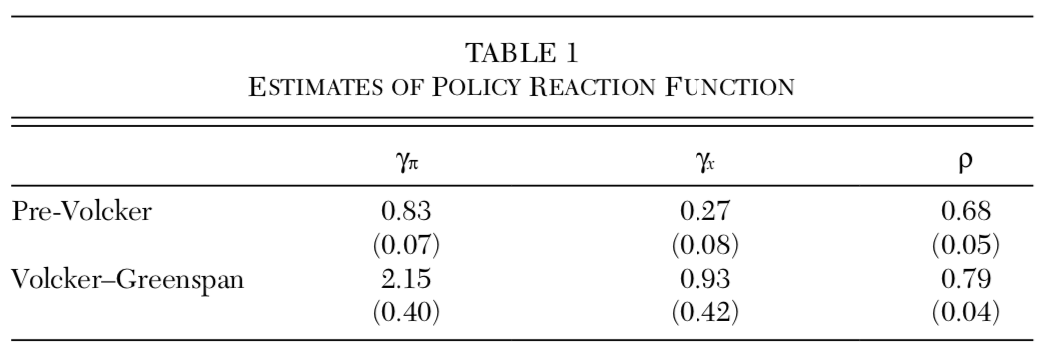
\includegraphics[scale=0.5]{../../Readings/Images/CCG1999taylor.png}	
%	\end{center}
% \end{itemize}
%\end{frame}
%
%
%\begin{frame}
%\frametitle{Volcker-Greenspan Policy and the Principles}
%\begin{center}
%	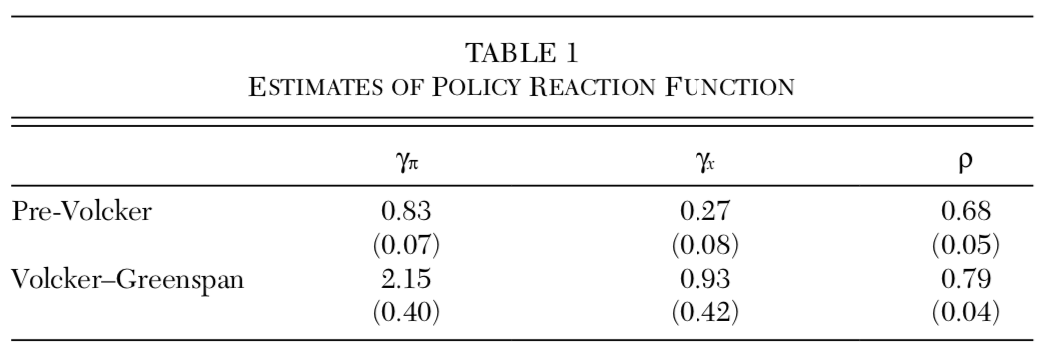
\includegraphics[scale=0.5]{../../Readings/Images/CCG1999taylor.png}	
%	\end{center}
%\begin{itemize}
%	\item Volcker and Grenspan aggressively follow Taylor principle.
%	\item Explicit inflation target of 2\% as use $\bar{\pi}=2\%$.
%	\item Try to figure out type of shock. For example, in 1990s with high productivity-driven growth, don't raise rates.
%	\item Next class: Should we adopt rules like this? Or other rules?
% \end{itemize}
%\end{frame}

\end{document}